% -*-latex-*-
% Document name: /u/macleod/gl/map3d-docs/notes/todolist.tex
% Creator: Rob MacLeod [macleod@cvrti.utah.edu]
% Creation Date: Mon Jul 30 10:19:24 2001
% Last update: Tue Oct 30 20:32:56 2001 by Rob MacLeod
%    - added more goodies\ldots{}
% Last update: Sun Apr 20 13:11:50 2003 by Rob Macleod
%    - reworked the list in time for the summer season 2003!
%%%%%%%%%%%%%%%%%%%%%%%%%%%%%%%%%%%%%%%%%%%%%%%%%%%%%%%%%%%%%%%%%%%%%%
\documentclass[11pt]{article}
\usepackage[]{html}
\usepackage[]{epsfig}
\textheight 9.5in
\textwidth 6.5in
\topmargin -.5in
\oddsidemargin 0in
\setlength{\parskip}{\smallskipamount}
\newcommand{\eg}{{\em e.g.,}}
\newcommand{\ie}{{\em i.e.,}}
\newcommand{\etc}{{\em etc.,}}
\newcommand{\etal}{{\em et al.}}
\newcommand{\degrees}{{$^{\circ}$}}
\newcommand{\splitline}{\begin{center}\rule{\columnwidth}{.7mm}\end{center}}
%% Usage:  \comm{Name}{Remarks}
\newcommand{\comm}[2]{\bigskip
                      \begin{tabular}{|p{11cm}|}\\\hline
                      \multicolumn{1}{|c|}{{\bf Comment by #1}}\\ \hline
                      #2\\ \hline
                      \end{tabular}
                      \bigskip }
\newcommand{\map}{\emph{map3d}}
\newcommand{\mapgl}{\emph{map3dGL}}
%%%%%%%%%%%%%%%%%%%%%%%%%%%% Setting to control figure placement
% These determine the rules used to place floating objects like figures 
% They are only guides, but read the manual to see the effect of each.
\renewcommand{\topfraction}{1.0}
\renewcommand{\bottomfraction}{.9}
\renewcommand{\textfraction}{0}
\setcounter{topnumber}{100}
\setcounter{bottomnumber}{100}
\setcounter{totalnumber}{100}


%%%%%%%%%%%%%%%%%%%%%%%%%%%%%%%%%%%%%%%%%%%%%%%%%%%%%%%%%%%%%%%%%%%%%%
\begin{document}


%%%%%%%%%%  Figures used in this file %%%%%%%%%%%%%%%%%%%%%%%%%%%%%%%%
%begin{latexonly}
  \newcommand{\surfcompare}%
  {\centerline{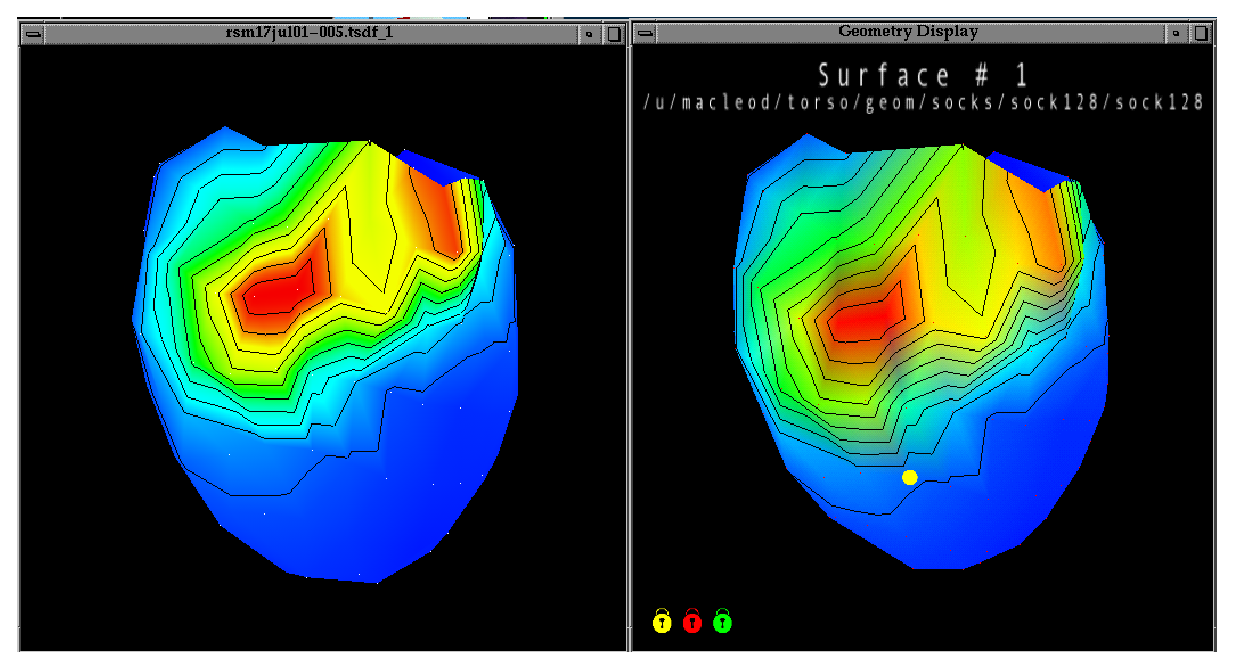
\epsfig{file=figures/map3d-comp1.ps,width=\columnwidth}}}
%end{latexonly}
\begin{htmlonly}
  \newcommand{\surfcompare}{%
  \htmladdimg[align=top,width=1053,alt="compare color mapping"]
  {figures/map3d-comp1.gif}}
\end{htmlonly}
%%%%%%%%%%%%%%%%%%%%%%%%%%%%%%%%%%%%%%%%%%%%%%%%%%%%%%%%%%%%%%%%%%%%%%
\newcommand{\X}[1]{#1\index{#1}}
\thispagestyle{empty}
\title{To Do List for map3d}
\author{Rob MacLeod and Bryan Worthen}
\date{\today}
\maketitle
%\newpage

\tableofcontents
\newpage

\section{Intro}

Here is what we hope will be a dynamic list of needs, wishes, and dreams for
\map{}.  The latest version 6 is a big improvement, and we are almost 
to the capabilities of the old \mapgl{} and have many new ones that
\mapgl{} will never enjoy.

\section{The Lists}

\subsection{Bugs that (may still) need fixn'}

\begin{enumerate}
  \item Nothing; the program is perfect!  (See bugzilla to dispell this
  illusion).
\end{enumerate}


\subsection{Rob's and Bryan's Top less-than-or-equal-to-20 List}

From the list below, here are our current top picks for things to do.  This
list, last updated on \today{}, lists first a number of ``small''
items, and then a few of the larger pieces we would like to tackle in the
near future.  See the more detailed list and the background sections below.

\begin{enumerate}
  \item Release source code version of map3d; include all necessary
    libraries and some documentation about how to make the program.
    Especially, make it clear that we have no facility to support changes;
    people can send things to us but we will have to evaluate their value
    before merging with the release version.
  \item Allow coloring of the nodes to match value.
  \item Allow some control over the number of significant digits get
    displayed when marking values on nodes or in scale bar.
  \item Add support for creating visualization geometry from a landmark
    file. 
  \item Add support for labels in landmark file.
  \item In reponse to another of Ed Ciaccio's comments, we should find a
    way to recycle the colors for data sets that span a large range,
    typically of activation times.  This arises when \map{} sees
    multiple beats in a single data file and the user wishes to see
    activation times for the series.  The solution Ed suggested was to
    reuse the colors.  What we need to figure out is how to control this
    and let the user determine what range of data values maps to each pass
    through the colors.   
 
  \item It may be time to consider a new interface to the clipping plans;
    as a start, we could have one clipping plane appear by default in the
    x-y screen plane, i.e., always cut the object at z=0 relative to the
    screen.  Then the other could do the same in another plane, perhaps
    x-z.  And perhaps we need some other way to control the plane, perhaps
    rotate it rather than the object?  Ideas?

  \item Continue to develop the visualization of time series attributes,
    \eg{} activation and recovery times together with time signals.

  \item Play with state saving and sript generation (Rob)
  \item Multiseries data file in .mat files
  \item Some features do not indicate their state i.e., whether it is
    turned on or not. (Bryan)
  \item Test: function to parse filenames and extract the experiment
    data and run number, which is encoded into the filenames for all tsdf
    files.  Then use this information where we do labelling. (RSM)
  \item Add iconify/maximize for all surfaces at
        once rather than each surface 
  \item Put the arrows on landmark fibers.  (status??)
  \item Investigate some new color maps that have less green/yellow and use
    more colors in their place.
  \item Support for script writing in which the user can save  current
    settings and layout in a script file for rerunning or editing.  This
    needs more testing and perhaps some user driven selection of content;
    it is a little too inclusive at present.

%  \item Restore support for reading multiple pot files, either with
%          wildcard or a series of files with numbered filenames.
%  \item Slave scaling between surfaces.
%  \item Make sure channel indirection works (I think I found a case where
%        it's buggy).  Also reset display of channel numbers to begin with
%        1 rather than 0.
%  \item Program keypad to control display--come up with a scheme
%        that works on a laptop too.
%  \item Capture screen contents and save in image file format. (halfway)
%  \item Update overview of map3d on the SCI website
%  \item update text on download page (refers only to CVRTI)
%  \item download for mac labels on required/recommended/options elements
%    need updating
%  \item figure out how to make the Mac version launch with double click.
%%   \item Make MATLAB data files from .tsdf  (Rob)
%%   \item (Done)Update test scripts to include .tsdf files
%%  \item Add to the scaling menu the option to set fixed contour spacing and
%%       allow user to enter and edit the spacing value. (JR)
%%   \item Allow the user to select one time signal and make it the reference
%%     against which all others are displayed.  This involves subtracting the
%%     value of the selected lead from all other leads for each time instant.
%%     We also need to be able to go back to the default condition, with the
%%     reference set of zero so must perform the subtract and yet still keep
%%     track of the referece time signal so we can add it back later.
%%  \item Add slave scaling to menus and group scaling to command line
%%  \item Test writing geom file after applying transform to existing geometry. 
%%  \item draw lines between RMS windows in dialog window
%%  \item make horiz colorbar labels "line up" with contours; make horizontal
%% color bar use less vertical space
%%   \item As a user option, add to the time signal window, the current data
%%     filename (in text) and the state of the scaling (true, symmetric, or
%%     separate).    
%  \item Apply depth queuing (fog) to labels, e.g., node numbers
%  \item Remove exit from readgeomfile (Rob)
%  \item Remove clobber question from geom file overwrite (Rob)
%  \item Remove datapath from inner workings
%  \item Get geom window saving working in windows
%  \item Tweaking the state saving and script composing support
%  \item Local version of necessary libs for map3d (Bryan is working on SCI
%  version, Rob on CVRTI)
%  \item Allow user to toggle visibility of the scale bars--one should be
%        able to turn then on and off as need, much like a time signal
%        window. 
%  \item Interactive control of sizes for fonts and other markings--user
%        selects which attribute to alter and then the keypad +/- keys can
%        adjust this. Likewise, set resolution of zoom steps.
%  \item Add touch-up controls for making figures from displays (thicker lines,
%        fewer colors, etc.)
%  \item Getting node and element information by picking. (test)
%  \item Test previous problems with independent rotation of surfaces and
%    then storing the transformed geometries to a new file.
%  \item Window attributes-->Size: remove the present options and replace
%        them with: fixed aspect ratio and variable aspect ratio and
%        then provide a list of standard window sizes like 400 by 400,
%        640 by 480, 1024 by 768, etc.
%  \item Add some control of near and far planes for depth cueing.
\end{enumerate}

\subsection{Larger items}

\begin{enumerate}
%  \item Complete support for MATLAB files.
%  \item Getting Mac OSX version working.
%%   \item Support user creation of animations, at least through dumping
%%     of a series of image files for subsequent conversion and ideally by
%%     means of remote control. (Bryan)
%%   \item Resolution of portability problems with tsdfc library and reading
%%     container files. (J.R.)
%  \item Save state of program in \texttt{.map3drc} file and read it again
%    at launch time.
%  \item Save script of current layout of map3d so that user can run again,
%    perhaps even edit the script to generalize.
  \item Restore use of report level throughout the code and allow user to
        select it from a menu.
%%   \item Is there was way to get map3d to save gif or jpg files?  I am
%%     liking png less and less as I use it.  I would most like if the
%%     user could select the format and that it included rgb when on the
%%     SGIs. 
%  \item Try and make color mapping better match \map3dgl{} version.  See
%    Figure~\ref{fig:surfcompare} for a comparison.
\end{enumerate}

\subsection{Release Documentation list}
\begin{enumerate}
\item (Done)Mac installation
\item (Done)Frame control(set time to zero)
\item (Done)Reference leads
\item (Done)Pick Window more detailed info toggle
\item Matlab file format
\item (Done) Matlab file usage
\item (Done) 'w' key to save image quickly
\item (Done) more details on image saving dialog
\item (Done) CTRL+SHIFT can be substituted for ALT
\item (Done) script saving
\item (Done) state saving
\item (Done) new version of gouraud shading (textures) + method of reverting
\item (Done) bug fixes: image saving (and many unknown ones) 
\end{enumerate}



\section{The Rest of the List}

Here is a list in outline form of some more things in the waiting list.
See the background sections below for more details.

\subsection{Display}

\begin{enumerate}
%%   \item Color mapping on new \map{} does not match that on the old.  See
%%         Figure~\ref{fig:surfcompare} for a comparison.
  \item Dynamic waterfall plots of two-dimensional datasets on irregular
        grids. 
  \item ``Video display'' options to thicken lines and increase font
        sizes or remove unnecessary lettering.
  \item Provide user options, via the command line and eventually a menu to
        enter text strings to show in the displayed material for the
        surface windows.  This would allow the user to make some labels for
        the displays.
  \item Vector field visualization.
  \item Stereo viewing and VR control.
\end{enumerate}

\begin{figure}[htb]
  \begin{makeimage}
  \end{makeimage}
\surfcompare
\caption{\label{fig:surfcompare} Comparison of color mapping between old
(left) and new (right) map3d.}
\end{figure}

\subsection{Controls}

\begin{enumerate}
%  \item Dials support
%  \item Keypad controls as in \mapgl{}
%%   \item Support for 3D manipulation device; used to be dial box but now the
%%         3D trackball  is what SGI offers.
  \item Window placement at start up or when launching new time series
        window. 
%%   \item Add more picking options, \eg{} selecting points, elements,
%%         etc. for interrogation.  Mark the last selection from picking.
%%   \item Dynamic pull down menus so that we can mark settings as on or off.
%  \item Add in geometry controls, \eg{} triangulating, flipping
%        triangles, moving landmarks.
%  \item UI, \eg{} qt, \htmladdnormallink{www.trolltech.org} 
%        {http://trolltech.gtk.org}
%        as interface to controls (scaling, contour number and/or spacing,
%        colors and sizes, and reading new data during \map{} session.
%  \item Settings files to keep your favorite settings around for the next
%        time--save state settings for restarting.
%  \item Interactive keyboard control of font size rather than via menu;
%        this is especially necessary for the label size; whenever a label
%        is on the nodes, then the + and - keys on the keypad should control
%        the font size in fairly small increments.
  \item Control of lighting model
  \item Remote control of animations.
%%   \item In borderless window mode, we need to be able to adjust the size of
%%         the individual sub windows and display the new size and location
%%         interactively. 
\end{enumerate}

\subsection{Input/output}

  \begin{enumerate}
%    \item Restore support for reading multiple pot files, either with
%          wildcard or a series of files with numbered filenames.
%    \item Read all surfaces from a .geom file.
    \item When saving the mesh, there appears to be a bug in the way the
          meshes are saved; the main need here is to adjust a mesh and then
          save it with that adjustment.  The ambiguity arises with what we
          mean by adjustment.  One would like to be able to move one surface
          relative the other and then save the moved mesh with just the
          transformations applied relative to the other geometry.  It
          appears now that moving just one surface and save the results
          leads to both surfaces being transformed--and even then, their
          relative position is not preserved.
%    \item Capture screen contents and save in image file format
%    \item Read container files of time series data
%    \item Window incoming data, via UI like Formslib in \map3dgl{}.
%    \item Save transformed geometry.
%    \item Update data on display during execution.
%    \item Saving sequences of images for animations.
    \item Use feedback mode to capture screen contents as vector based
          postscript.
    \item When specified without extension, the program should look for
          sensible file extensions and complete them if possible; right now
          it does this for the first surface of a multisurface plot but
          then fails on the others.
  \end{enumerate}

\subsection{Documentation}

  \begin{enumerate}
    \item Make some new screen dumps from the scalar display for the
          manual. 
%    \item Make screen shots of color and size selection windows.
%    \item Manipulation of borderless windows--make sure docs reflect
%          reality. 
%    \item Does this work now?>  If so, documebt,  Window attributes-->Size:
%          remove the present options and replace them with: fixed aspect
%          ratio and variable aspect ratio and then provide a list of
%          standard window sizes like 400 by 400, 640 by 480, 1024 by 768,
%          etc.
    \item Check on the controls available for landmarks and update
          controls.\TeX{} accordingly.
  \end{enumerate}

\subsection{Miscellaneous}
\label{sec:misc}

\begin{itemize}
  \item Display of text in main window:
        \begin{itemize}
          \item When only geometry available, print the geometry file name.
          \item When potentials and geometry available, print the data file
                name. 
          \item If more than on surface present, but only geometries, if
                the surfaces all came from the same .geom file, print that;
                if they come from 2-3 files, print all of them; if more
                than 3 files, print first with a ``+ others'' below it.
          \item If more than one surface present with potentials, try and
                print all the potentials filenames (may need to eventually
                limit this but it should not be a real problem).
          \item Make sure to parse all filenames so that they show either
                no path or at most the last part element.
        \end{itemize}
  \item Window attributes-->Size: remove the present options and replace
        them with: fixed aspect ratio and variable aspect ratio and
        then provide a list of standard window sizes like 400 by 400,
        640 by 480, 1024 by 768, etc.
%  \item map3d without arguments should generate the usage string to the
%        user
%  \item restore use of report level throughout the code and allow user to
%        select it from a menu.
%  \item remote control of the animations and user interventions for making
%        videos 
\end{itemize}


\section{Some background}

%% \subsection{Borderless window mode}

%%   There does not seem to be a clear notion of how to set the large parent
%%   window for this mode.  There seems to be a fixed size of parent window
%%   that will no grow even if the contents of the window are larger that its
%%   total.  For example, I specific two windows with -as and then also a
%%   borderless window.  The result is a mess in that the -as addresses seem
%%   to be ignored or at best are relative to the parent window.  

%%   What I (Rob) think should happen is that we scan all the specs in the -as
%%   parameters and then is we have borderless window mode always define the
%%   parent window to include the subwindows at the right location on the
%%   screen.  For example, with 
%%   \begin{verbatim}
%%   $MAP3D -nw -b -f ${GEOM}/25feb97_sock.fac \
%%         -as 100 400 100 400 \
%%         -p ${DATA}/cool1-atdr_new.data@1 -s 1 1000 \
%%         -ch ${GEOM}/sock128.channels \
%%         -f ${GEOM}/25feb97_sock_closed.geom \
%%         -as 401 700 100 400 \
%%         -p ${DATA}/cool1-atdr_new.data@2 -s 1 1000\
%%         -ch ${GEOM}/sock128.channels
%%   \end{verbatim}

%%   we should have a parent window with size for the two subwindows, plus
%%   the scaling windows, and place the subwindows where they want to be on
%%   the screen.  So the rectangle of the parent window would be at least 100
%%   700 100 400 plus some space for the scaling windows.  They should appear
%%   wherever makes sense of there is space.  If there is no space, then leave
%%   them out.
  
%%   Also note that with the above specs, there is a one-pixel wide space
%%   between the subwindows, even though the left address of one and the right
%%   address of the other are adjacent.  I (Rob) think we should use a
%%   one-based addressing with 1,1 in the lower left hand corner.  I suspect
%%   that somewhere there is a one shift happening in one place and not in
%%   another.


\subsection{Scaling options}
\label{sec:scaling} 

There is a wide variety of options available for mapping scalar values to
colour and contour levels.  One can picture the process as based on four
facets: 

\begin{description}
  \item [Extrema: ] the extrema of the data and the selected colour maps
        determine the basic parameters of how value maps to color.  \map{}
        maintains a detailed list of data extrema organized both by time
        signal, time instant and by surface.  Thus it is possible to determine
        extrema based on just the most local of conditions---a particular
        frame and surface---or by more global conditions---the full range
        of frames or the full set of surfaces.
  \item [Scaling function: ] the mapping between value and color occurs
        according to some mathematical function, the simplest of which
        is linear.   The scaling function uses the selected extrema and
        describes a complete mapping between value and color.
  \item [Mapping: ] by scale mapping, we mean how the translation from
        value to color treats positive and negative values.  We may choose
        to map uniformly between the extrema or to apply different
        extrema or functions to the positive and negative values.
  \item [Color maps: ] the color displayed for a particular scalar value
        depends on the actual range of colors and their order in the color
        map.
\end{description}

\map{} can adjust all four facets of the scaling to create a wide range of
displays.  We chose to limit some of these options, however, in an effort
to create reproducible displays that reflect standard within the field.  Of
course, we chose our field, electrocardiography, as the basis, a fact for
which we make no apologies and simply encourage others to make similar
choices for their own field and implement \map{} accordingly.  Subsequent
versions of \map{} will support this flexibility.

Below are the specific choices that \map{} offers to control data scaling
and display
\begin{description}
  
  \item[Scale range] \map{} supports several selections of range over
        which to look for extrema.  In {\em local\/} range, only the data
        presently visible 
        are scanned for extrema---this is the default.  In the full {\em
        global\/} range, all the data in the entire dataset are used, even
        those not presently visible on the display.  In between these
        cases, one can have global in time and local in space, \ie{} we
        scale each surface separately but use all time values for that
        surface.  Or one can 
        select local in time and global in space, in which \map{} scans all
        surfaces for the data extrema, but for each time instant separately
        The {\em user\/} scaling scope uses the current user-selected
        values for maximum and minimum for the scaling (see {\tt -pl} and
        {\tt -ph} input parameters.
        
  \item[Scale function] The scale model describes the way in which scalar data
        are mapped to colours (or contours).  The present choice is linear,
        but the next version of \map{} will include: \textbf{linear} model,
        which simply maps the data to a range of colours in a completely
        linear fashion, \ie{} \mbox{$colour = K \phi$}; the
        \textbf{logarithmic} model, which highlights the lower level data
        values at the cost of poorer resolution at the higher levels \ie{}
        \mbox{$colour = A\log(\phi) + B$}; and the \textbf{exponential}
        model, which does the opposite, compressing the smaller levels and
        expanding the higher ones to span a wider colour range, \ie{}
        \mbox{$colour = A e^{B\phi}$}.

  \item[Scale Mapping] There are several different ways to manage
        the way positive and negative data are treated in the scaling
        transformations in \map{}.  The current version supports the
        simplest, or {\em true\/} mapping, in which the data are used as
        they are with no consideration of positive or negative values---the
        color map spreads evenly across the range of the extrema.
        Subsequent versions will support the {\em symmetric\/} scale
        mapping, which sets the positive and negative extrema
        symmetrically---the larger (in the absolute value sense) determines
        both maximum and minimum data values.  Also to appear in the net
        version is the {\em separate\/} scale mapping, in which the
        positive and negative extrema are treated completely
        separately---`half' the colours (and contours) are used for the
        positive values, half for the negative values.  This is equivalent
        to producing maps with the same number of contours for both
        positive and negative values, even when the positive data have a
        different absolute maximum value than the negative data.

  \item[Contour spacing] the contour values are a function of the data and
        the user selection of scale range, model, and mapping (see following
        items).  Fundamentally, the user selects between contour spacing
        based on the number of contours selected or based on fixed spacing
        between contours.  The actual result depends, in turn, on the range
        of data values and the desired mapping between value and colour.
\end{description}
  


\end{document}
